% !TEX program = xelatex
\documentclass[aspectratio=169]{beamer}
\usepackage{ucasminimal}

\title{College Beamer\\Presentation Themes}
\subtitle{Using \LaTeX{} to prepare slides}
\author{}
\date{Created 6 July 2026}

\begin{document}

\maketitle

\begin{frame}
  \vspace*{1.25cm}
  This template is a secondary creation of
  the \bhref{https://www.overleaf.com/latex/templates/sintef-presentation/jhbhdffczpnx}{SINTEF Presentation}
  template.

  Following is a brief introduction to using \LaTeX{} and beamer to prepare
  slides.

  This template is released under
  \bhref{https://creativecommons.org/licenses/by/4.0/}{Creative Commons CC BY 4.0}
  license.
\end{frame}

\section{Introduction}

\begin{frame}{Beamer for SINTEF slides}
  \begin{itemize}
    \item We assume you can use \LaTeX; if you cannot,
      \bhref{https://en.wikibooks.org/wiki/LaTeX}{you can learn it here}
    \item Beamer is one of the most popular and powerful document classes for
      presentations in \LaTeX
    \item Beamer also has a detailed
      \bhref{https://ctan.org/pkg/beamer}{user manual}
    \item Here we present only the most basic features to get you up to speed
  \end{itemize}
\end{frame}

\begin{frame}{Beamer vs. PowerPoint}
  Compared to PowerPoint, using \LaTeX{} is better because:
  \begin{itemize}
    \item It is not What-You-See-Is-What-You-Get, but
      What-You-\emph{Mean}-Is-What-You-Get:\\
      you write the content, the computer does the typesetting
    \item Produces a \texttt{pdf}: no problems with fonts, formulas, or program versions
    \item Easier to keep consistent style, fonts, highlighting, etc.
    \item Math typesetting in \TeX{} is the best:
      \begin{equation*}
        \mathrm{i}\hbar\frac{\partial}{\partial t}\Psi(\mathbf{r},t)
        = -\frac{\hbar^2}{2m}\nabla^2\Psi(\mathbf{r},t)
        + V(\mathbf{r})\Psi(\mathbf{r},t)
      \end{equation*}
  \end{itemize}
\end{frame}

\section{Editing}

\begin{frame}[fragile]{Selecting the Class}
  After the last update to the graphic profile, the \texttt{sintef} theme for
  Beamer has been updated into a full-fledged class. To start working with
  \texttt{sintefbeamer}, start a \LaTeX{} document with the preamble:

  \begin{ucascodebox}{Minimum Beamer Document}
    \ucascodeline{1}{\codebs documentclass\{beamer\}}
    \ucascodeline{2}{\codebs begin\{document\}}
    \ucascodeline{3}{\codebs begin\{frame\}\{Hello, world!\}}
    \ucascodeline{4}{\codebs end\{frame\}}
    \ucascodeline{5}{\codebs end\{document\}}
  \end{ucascodebox}
\end{frame}

\begin{frame}[fragile]{Title page}
  To set a typical title page, you call some commands in the preamble:

  \begin{ucascodebox}{The Commands for the Title Page}
    \ucascodeline{1}{\codebs title\{Sample Title\}}
    \ucascodeline{2}{\codebs subtitle\{Sample subtitle\}}
    \ucascodeline{3}{\codebs author\{First Author, Second Author\}}
    \ucascodeline{4}{\codebs date\{Defaults to today's\}}
  \end{ucascodebox}

  You can then write out the title page with \verb|\maketitle|.
  You can set a different background image by changing the background path
  before calling \verb|\maketitle|.
\end{frame}

\begin{frame}{Writing a Simple Slide}
  \framesubtitle{It's really easy!}
  \begin{itemize}
    \item A typical slide has bulleted lists
  \end{itemize}
\end{frame}

\begin{frame}{Writing a Simple Slide}
  \framesubtitle{It's really easy!}
  \begin{itemize}
    \item A typical slide has bulleted lists
    \item These can be uncovered in sequence
  \end{itemize}
\end{frame}

\begin{frame}[fragile]{Writing a Simple Slide}
  \framesubtitle{It's really easy!}
  \begin{itemize}
    \item A typical slide has bulleted lists
    \item These can be uncovered in sequence
  \end{itemize}

  \begin{ucascodebox}{Code for a Page with an Itemised List}
    \ucascodeline{1}{\codebs begin\{frame\}}
    \ucascodeline{2}{\hspace*{1.8em}\codebs frametitle\{Writing a Simple Slide\}}
    \ucascodeline{3}{\hspace*{1.8em}\codebs framesubtitle\{It's really easy!\}}
    \ucascodeline{4}{\hspace*{1.8em}\codebs begin\{itemize\}[\textless{}+->]}
    \ucascodeline{5}{\hspace*{3.6em}\codebs item A typical slide has bulleted lists}
    \ucascodeline{6}{\hspace*{3.6em}\codebs item These can be uncovered in sequence}
    \ucascodeline{7}{\hspace*{1.8em}\codebs end\{itemize\}}
    \ucascodeline{8}{\codebs end\{frame\}}
  \end{ucascodebox}
\end{frame}

\begin{frame}[fragile]{Adding images}
  Adding images works like in normal \LaTeX:

  \begin{columns}[T,totalwidth=\textwidth]
    \begin{column}{0.62\textwidth}
      \begin{ucascodebox}{Code for Adding Images}
        \ucascodeline{1}{\codebs usepackage\{graphicx\}}
        \ucascodeline{2}{\codebs includegraphics[width=\codebs textwidth]\{gallery/img.jpg\}}
      \end{ucascodebox}
    \end{column}
    \begin{column}{0.32\textwidth}
      \vspace{0.18cm}
      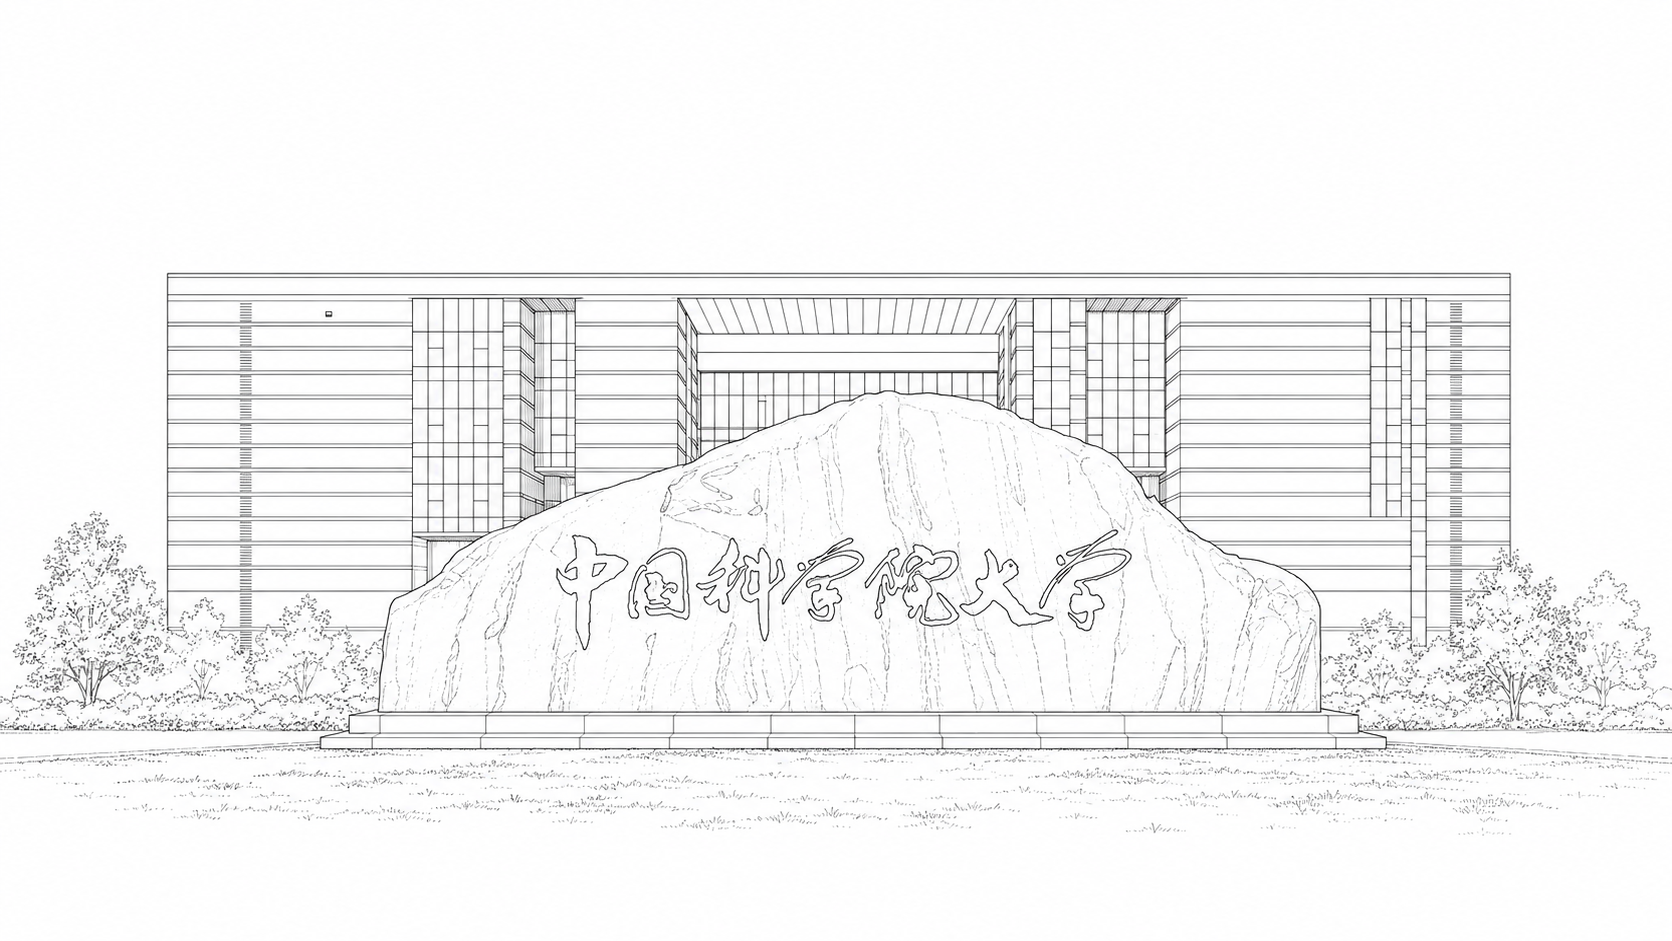
\includegraphics[width=\linewidth]{assets/ucas-background.png}
    \end{column}
  \end{columns}
\end{frame}

\begin{frame}[fragile]{Splitting in Columns}
  Splitting the page is easy and common; typically, one side has a picture and
  the other text:

  \begin{columns}[T,totalwidth=\textwidth]
    \begin{column}{0.58\textwidth}
      This is the first column
    \end{column}
    \begin{column}{0.34\textwidth}
      And this the second
    \end{column}
  \end{columns}

  \begin{ucascodebox}{Column Code}
    \ucascodeline{1}{\codebs begin\{columns\}}
    \ucascodeline{2}{\hspace*{1.8em}\codebs begin\{column\}\{0.6\codebs textwidth\}}
    \ucascodeline{3}{\hspace*{3.6em}This is the first column}
    \ucascodeline{4}{\hspace*{1.8em}\codebs end\{column\}}
    \ucascodeline{5}{\hspace*{1.8em}\codebs begin\{column\}\{0.3\codebs textwidth\}}
    \ucascodeline{6}{\hspace*{3.6em}And this the second}
    \ucascodeline{7}{\hspace*{1.8em}\codebs end\{column\}}
    \ucascodeline{8}{\hspace*{1.8em}\textcolor{UCASCodeMuted}{\% There could be more!}}
    \ucascodeline{9}{\codebs end\{columns\}}
  \end{ucascodebox}
\end{frame}

\begin{frame}{Fonts}
  \begin{itemize}
    \item Fonts should be readable.
    \item There are good ones:
      \begin{itemize}
        \item Serif fonts only with high-definition projectors
        \item Sans-serif fonts are usually safer
      \end{itemize}
    \item There are also not so good ones:
      \begin{itemize}
        \item Avoid monospace for normal text
        \item Avoid gothic, calligraphic or weird fonts
      \end{itemize}
  \end{itemize}
\end{frame}

\begin{frame}{Look}
  \begin{itemize}
    \item Theme color options are concentrated in the style file; this UCAS
      version uses \ctexttt{\#174994}.
    \item The theme keeps a light normal page and dark section/backmatter pages,
      following the visual rhythm of the reference demo.
    \item To insert a final slide, use the provided \texttt{\textbackslash{}QApage} command.
    \item The aspect ratio is set by Beamer; this demo uses
      \texttt{aspectratio=169}.
  \end{itemize}
\end{frame}

\section{Summary}

\begin{frame}{Good Luck!}
  \begin{itemize}
    \item Enough for an introduction! You should know enough by now
    \item Adapt the examples to suit your own presentation
  \end{itemize}
\end{frame}

\QApage

\end{document}
